\documentclass[12pt]{article}
\usepackage[utf8]{inputenc}
\usepackage{graphicx}
\usepackage{biblatex}
\usepackage{titlesec}
\usepackage{geometry}
\usepackage{setspace}
\usepackage{minted}
\usepackage{biblatex}
\usepackage{listings}
\usepackage{tocloft}
\usepackage{longtable}
\usepackage{placeins}
\geometry{
 a4paper,
 left=35mm,
 top=25mm,
 right=25mm,
 bottom=25mm,
 }
\setstretch{1.5}
\addbibresource{biblio.bib}
\bibliography{reference}
\begin{document}
\graphicspath{{./pictures/}}
\titlelabel{\thetitle.\quad}
\renewcommand*\contentsname{Obsah}
\renewcommand{\bibfont}{\small}
\renewcommand{\thesection}{\Roman{section}} 
\renewcommand{\thesubsection}{\thesection.\Roman{subsection}}
\renewcommand{\thesubsubsection}{\thesubsection.\Roman{subsubsection}}
\renewcommand\listoflistingscaption{Seznam příloh}
\renewcommand{\listingscaption}{Příloha}
\addtolength{\cftsecnumwidth}{2pt}
\addtolength{\cftsubsecnumwidth}{10pt}
\addtolength{\cftsubsubsecnumwidth}{12pt}
\begin{titlepage}
\begin{center}
    \vspace{2,5cm}
    \textbf{\Large Gymnázium, Praha 6, Arabská 14}\par
    \Large Obor Programování\par
    \vspace{2cm}
    \textbf{\Huge Maturitní práce}\par
    \vspace{2cm}
    \textbf{\Huge Alternativní Strava.cz klient}\par
    \vspace{2cm}
    
\includegraphics[]{logo}\par
    \vfill
   \Large Jakub Turek \hfill Duben 2024
   
    
     
\end{center}
\end{titlepage}
\newpage{}
\thispagestyle{empty}
\mbox{}
\vfill
Prohlašuji, že jsem jediným autorem tohoto projektu, všechny citace jsou řádně označené a všechna použitá literatura a další zdroje jsou v práci uvedené. Tímto dle zákona 121/2000 Sb. (tzv. Autorský zákon) ve znění pozdějších předpisů uděluji bezúplatně škole Gymnázium, Praha 6, Arabská 14
oprávnění k výkonu práva na rozmnožování díla (§ 13) a práva na sdělování díla veřejnosti (§ 18) na dobu časově neomezenou a bez omezení územního rozsahu.
\newline
V Brandýse nad Labem dne 2.4.2024 \hfill Jakub Turek
\newpage{}
\thispagestyle{empty}
\section*{Anotace}
Následující práce pojednává o tvorbě alternativní klientské aplikace pro sloužící pro správu objednávek jídel v jídelnách, a to jak v podobě webové aplikace, tak desktopové aplikace pro operační systémy Linux a Windows s využitím frameworku Tauri a programovacího jazyka Rust pro tvorbu backendu a funkcionality samotné aplikace a frameworku SvelteKit a scriptovacího jazyka TypeScript pro tvorbu frontendu a uživatelského rozhraní desktopové aplikace. Výsledná klientská aplikace zachovává funkcionalitu oficiální aplikace a rozšiřuje ji o možnost automatické správy objednávek dle uživatelem specifikovaných preferencí (oblíbené pokrmy, obsah konkrétních alergenu, atd.). 
\section*{Abstract}
The main topic of following thesis is creation of alternative client application for Strava.cz webappliction, which serve for management of orders of dishes in different cantines in form of webapplication a desktop application for Linux a Windows with use of Tauri framework and Rust programming language for webapplication backend a desktop application and SvelteKit with TypeScript for webapplication frontend and desktop application user interface. This alternative client application preserve funcionality of official aplication and extends it with automatic management of orders based on user specified preferences (favourite dishes, containsed allergens, etc.).
\newpage
\setcounter{page}{1} 
\renewcommand{\baselinestretch}{1.4}\normalsize
\tableofcontents 
\renewcommand{\baselinestretch}{1.5}\normalsize
\newpage
\section*{Úvod}
Následující práce pojednává o tvorbě alternativní klientské aplikace pro aplikaci Strava.cz sloužící pro správu objednávek v jídelnách. Z této oficiální aplikace aplikace získává data pomocí separátního web scarepru. Na jejich základě, společně se vstupem od uživatele, vytváří HTTP požadavky na oficiální aplikaci. Aplikace zároveň rozšiřuje oficiální aplikaci o možnost automatické správy objednávek na základě uživatelem definovaných předvolbe, například filtrování jídel dle obsažených alergenů, či seznamy oblíbených a neoblíbených jídel.

Aplikace zároveň je zároveň vytvořena s využitím frameworku Tauri pro programovací jazyk Rust, který umožňuje tvorbu desktopových aplikací s využitím webových technologií pro tvorbu uživatelského rozhraní, což umožňuje relativně snadnou tvorbu jak webové, tak desktopové verze aplikace bez nutnosti modifikovat vetší množství napsaného kódu, aplikace této výhody taktéž využívá a je tak dostupná jednak v podobě webové aplikace, tak jako desktopová aplikace pro Linux a Windows. Způsob implementace webové a desktopové aplikace bude popsán podrobněji v následujících kapitolách. Pro tvorbu frontendu webové aplikace a UI desktopové aplikace je použit framework SvelteKit a TypeScript.

Vzhledem k vysoké míře provázání mezi webovou a desktopovou verzí aplikace bude následující text pro přehlednost pojednávat o obou verzích aplikace společně a každá kapitola bude obsahovat informace o obou verzích.
\addcontentsline{toc}{section}{Úvod}
\newpage
\section{Použité technologie}
Následující kapitola pojednává o klíčových technologiích využitých při tvorbě projektu a stručně nastinuje formu jejich využití.
\subsection{Tauri}
Je sada nástrojů sloužící pro tvorbu desktopových aplikací v jazyce Rust s využitím webových technologii, primárně pro tvorbu uživatelského rozhraní. Integruje například také sadu nástrojů Wix od společnosti Microsoft sloužící pro vytváření instalátorů pro operační systém Windows\cite{wix} a další nástroje\cite{building}, které značně usnadňuje a uživatelsky zpříjemňuje distribuci výsledné aplikace, či systém závislostí umožnující snadnou integraci softwaru třetích stran potřebného pro běh programu. Přesné využití Tauri bude podrobněji popsáno v kapitolách zabíhajících se architekturou aplikace a klíčovými problémy 
\subsection{Actix}
Je webový framework pro programovací jazyk Rust, který nabízí základní implementaci funkcionalit potřebných pro vývoj webových aplikací (HTTP server, routing, atd.), doplněných o ekosystém dalších knihoven poskytujících funkce potřebné pro specifičtější případy užití. Zároveň poskytuje podporu pro přímé produkční nasazení výsledné aplikace, v případě tohoto projekt však samotná aplikace koncipovaná k nasazení společně s reverzní proxy Traefik\cite{actix}.
\subsection{Traefik}
Je reverzní proxy, jejíž hlavní výhodou, pro níž je použita i v tomto projektu, je vysoká míra integraci s technologiemi jako je Docker, kdy pak samotná proxy vyžaduje minimální manuální konfiguraci, kterou je možné provést prostřednictvími konfiguračních souboru Dockeru. Dále pak podporuje automatickou konfiguraci SSL\cite{autossl}\cite{traefik}.
\subsection{Tokio}
Tokio je knihovna poskytující asynchronní běhové prostředí pro jazyk Rust a zároveň usnadňuje asynchronních I/O operace (více vysokoúrovňová implementace), v případě tohoto projektu asynchronní komunikace po síti. Rust jako takový poskytuje podporu pro asynchronní programování avšak pro samotné přeložení a spuštění je třeba externí běhové prostředí, které umožní spuštění asynchronního kódu, které poskytuje právě Tokio\cite{tokio}.
\subsection{MongoDB}
Jedná se on o NoSQL, což znamená, že místo klasické struktury tabulek, jakou známe z SQL databází, jsou data ukládána do souboru BSON, binární forma formátu JSON, což usnadňuje například ukládání souboru. Databázi je také možno v rámci služby Atlas provozovat v cloudu, což přináší nejen snížení nároku na vlastní infrastrukturu a jednodušší údržbu, ale také některé pokročilé agregační funkce a real time vizualizaci jejich výsledků, které nejsou v běžné distribuci dostupné, tyto funkce tento projekt nevyužívá, aby bylo možné jeho databázi hostovat i mimo službu Atlas. Pro komunikaci s databází používá aplikace oficiální driver pro jazyk Rust bez jakéhokoliv objektového mapování.
\subsection{Fantoccini a Firefox}
Oficiální Strava.cz aplikace používá vykreslování na straně klienta, z tohoto důvodu je třeba jednotlivé elementy webu nejprve vykreslit, aby z nich web sacraper mohl získat potřebná data, samotný proces získávaní dat z oficiální aplikace bude popsán později v tomto textu. Pro účely vykreslení potřebných elementů webové aplikace je tedy používán webový prohlížeč v jeho headless verzi, která je ovládána prostřednictvím WebDriver protokolu, který umožňuje kontrolovat webový prohlížeč\cite{webdriver} a jehož implementaci pro jazyk Rust zajišťuje právě právě knihovna Fantoccini\cite{fantoccini}.
\subsection{SvelteKit}
SvelteKit je webový framework, který rozšiřuje knihovnu Svelte, která slouží pro tvorbu webového frontendu za použití komponent, o funkce potřebné pro vývoj plnohodnotné webové aplikace, jako je routing, práce se způsobem vykreslování, systém adaptérů pro různé typy nasazení (statický web, Node.js server, různé cloudové služby)\cite{adapters}. Na rozdíl od dalších frameworku, se kód aplikace vytvořené s pomocí Sveltu překládá do čistého JavaScriptu, který je následně vykreslí výslednou stránku\cite{sveltekit}. SvelteKit je v projektu použit pro tvorbu frontendu webové aplikace a současně UI desktopové aplikace, kdy je v obou případech použit stejný kód a liší se pouze komunikační vrstva mezi ním a zbytkem aplikace, podrobná implementace komunikačních vrstev bude popsáná v kapitole pojednávající o klíčových problémech.
\subsection{Tailwind CSS}
Tailwind CSS je CSS framework, ktrý využívá systému takzvaných "utility class", které vždy konfigurují určitý CSS styl a jejich vzájemnou kombinací se docílí požadovaného výsledku. Tailwind také automaticky optimalizuje výsledný soubor stylů, který bude po sestavení aplikace odesílán klientskému prohlížeči, aby nedocházelo ke zbytečnému zpomalování výsledné aplikace načítáním nevyužitých stylů\cite{tailwind}.
\newpage
\section{Struktura projektu}
Následující kapitola pojednává o struktuře aplikace, kdy stručně nastiňuje rozdělení projektu do několika větších komponent a popisuje jejich fungovaní.
Celkem je projekt rozdělen do celkem čtyř crate (název používaný Rustem pro jednotlivé balíčky kódu), ve třech případech se jedná o samostatné spustitelné programy, \textit{api}, spustitelný balíček obsahující backend webové aplikace, \textit{tauri-src}, balíček desktopové verze aplikace a \textit{startup-script}, jednoduchá konzolová aplikace zajištující fungování automatické správy objednávek. Poslední z balíčku je knihovní balíček obsahující funkcionalitu sdílenou mezi všemy výše zmíněnými spustitelnými balíčky, jako jsou datové struktury, implementace síťové komunikace, či získávání dat z výchozí aplikace. Poslední z komponent projektu je SvelteKit projekt sloužící jako frontend webové aplikace a zároveň jako uživatelské rozhraní pro aplikaci desktopovou.
\subsection{Strava klient}
Jak již bylo řečeno výše jedná se o knihovní balíček, který zajišťuje většinu klíčových funkcí projektu. Obsahuje jednak \textit{RequestBuilder}, který je implementován v souboru \textit{request\_builder.rs} a zajišťuje základní komunikaci prostřednictvím HTTP protokolu, na je zákldě ja implementován také \textit{StravaClient}, který nabízí vetší míru abstrakce pro pohodlné vytváření požadavků na originální aplikaci a získávaní dat z jejího API. Na jeho základě je implementovaná ještě jeho automatizovaná verze, která poskytuje stejné funkce s tím rozdílem, že k vytváření požadavků není využíván vstup od uživatele, jím definované předvolby a \textit {AutomaticClient} tak představuje základ fungování automatické správy objednávek.

V neposlední řadě knihovna obsahuje sdílené datové struktury používané pro zachování konzistence k reprezentaci dat napříč moduly a také k jejich serializaci při ukládaní do databáze. Podrobněji bude fungování jednotlivých částí popsáno v následující kapitole pojednávající o získávání dat a schématu databáze.
\subsection{Api}
Tento balíček představuje backend webové aplikace a kromě samotné implementace HTTP serveru vytvořeného s pomocí knihovny Actix, obsahuje tak implementaci komunikaci s databázi,která je implementována nad oficiálním driverem pro jazyk Rust prostřednictvím objektu \textit{DBClient}.

\begin{listing}[!ht]
\begin{longtable}{ |p{2.8cm}|p{1.4cm}|p{3cm}|p{2cm}|p{4cm}| }
\hline
\multicolumn{5}{|c|}{Struktura API webové aplikace} \\
\hline
Path& Method& Body& Query& Výsledek \\
\hline
/cantine\_history& GET& none& cantine\_id, query& vrátí seznam jídel v historii jídelny vyhovující vyhledávání\\
\hline
/login& POST&  \{jmeno:string, heslo:string, cislo:string, lang:string, zustatPrihlasen:bool\}& none& provede ověření identity uživatele \\
\hline
/logout& POST&  none& none& ukončí session s klientem - odhlášení \\
\hline
/user\_menu& GET&  none& none& vrátí jídelníček právě přihlášeného uživatele \\
\hline
/user\_settings& GET&  none& none& vrátí nastavení automatické správy objednávek přihlášeného uživatele \\
\hline
/user\_settings& POST& \{name:string, allergens:string[]\}& list, action& provede akci (add, remove,  replace) s nad daným atributem (allergens, blacklist, whitelist, strategy) \\
\hline
/order\_dish& POST&  \{id:string, status:bool\}& none& provede objednávku daného jídla \\
\hline
/save\_orders& POST&  none& none& uloží objednávky\\
\hline
/user\_status& GET&  none& none& vrátí zdali je uživatel přihlášen\\
\hline
/settings\_query& GET&  none& query, list& provede textové vyhledávání na zadaném list nastaverní (blacklist, whitelist, allergens)\\
\hline
\end{longtable}
\caption{Struktura API a stručný popis jeho fungování}
\end{listing}

Dále balíček obsahuje také \textit{CrawlerScript}, který slouží pro procházení oficiální aplikace a vytváření historie jídelen na základě jím získaných dat.

Co se samotné obsluhy příchozích požadavků, ta je realizována voláním funkcí implementovaných v rámci objektů \textit{StravaClient} a \textit{DBClient}, doplněných o správu session, na jejichž bázi je implementovaná autentizace uživatelů\cite{auth}, a na nich závislém stavu\cite{state} uloženého na serveru po dobu jejich existence (spojení mezi serverem a oficiální aplikací).

Tabulka výše znázorňuje strukturu a způsob fungování komunikačního rozhraní backendu webové aplikace.

\subsection{Desktopová aplikace}
Balíček \textit{src-tauri}, představuje samotnou desktopovou aplikaci, svým fungováním se v základech příliš neliší od backendu webové aplikace. S tím rozdílem, že v tomto případě není nutná zdaleka tak komplexní autentifikace a udržování stavu, jelikož je zde obsluhován vždy pomyslně obsluhován pouze jeden klient a dojde proto poze k odeslání autentizačního požadavku oficiální aplikaci a případně i backendu webové aplikace, je-li nutná komunikace s databází. Poté už dochází obdobně jako u webové verze k obsluze jednotlivých požadavků, kterými jsou v tomto případě události vyvolávané komunikační vrstvou aplikace prostřednictví api Tauri frameworku\cite{invoke}. 

\subsection{Script po spuštění}
Je jednoduchý spustitelný balíček, který slouží pro efektivní fungování automatické správy objednávek v desktopové verzi aplikace, kde dochází k jeho spuštění s každým zapnutím počítače a je tak zajištěno pravidelné spouštění automatizované správy objednávek. Tato funkce zatím automaticky funguje pouze ve verzi pro operační systém Windows, kde je pro spouštění aplikace při startu systému třeba pouze vložit její soubory do k tomu vyhrazené složky\cite{startup}.

\subsection{Frontend}
Poslední z větších komponent projektu je frontendová aplikace vytvořená s pomocí SvelteKit frameworku, která slouží jak jako frontend webové aplikace, tak jako uživatelské rozhraní její desktopové verze, z tohoto důvodu využívá aplikace metodu předrenderování jejích statických částí, které jsou pak za pomocí TypeScriptu doplněny o dynamický obsah vykreslený na straně klienta. Tento kompromis umožnuje velmi snadné znovupoužití frontendové aplikace jak pro webovou, tak desktopovou verzi, s nutností změnit jen minimální množství kódu.

Aplikace se zároveň skládá ze dvou hlavních částí, stránky s objednávkami, která obsahuje vetšinu funkcionality originální aplikace, umožňuje uživateli manuálně spravovat objednáky, zobrazovat zůstatek na účtě, procházet jídelníček jídelny a tak dále. Druhou z částí je stránka pro konfiguraci automatické správy objednávek, která umožňuje nastavení oblíbených a neoblíbených jídel, alergenů, které nesmí objednaná jídla obsahovat, či strategie automatické správy objednávek, kdy ve výchozím nastavení dochází pouze k rušení objednávek obsahující zakázané alergeny, či jídla vyskytující se na seznamu neoblíbených jídel. Ale je možná přepnout i na možnost, kdy jsou odhlášená jídla nahrazovaná alternativním možnosti, které vyhovují předvolbám a zároveň jsou upřednostňována oblíbená jídla před jídly ostatními, či automatickou správu zcela vypnout. Při vytváření obou seznamů jídel vybírá z historie jídel vařeních jídelnou v minulosti a přesouvá je na jím vytvářený seznam pomocí drag and drop mechaniky, či pouhým klikáním pro zachování kompatibility na mobilních zařízeních s dotykovou obrazovkou\cite{drag}. Ve všech seznamech jde zároveň vyhledávat pomocí vyhledávání implementovaného na úrovní databáze\cite{search} s pomocí regulárních výrazů\cite{regex}. Následující obrázek ukazuje rozložení stránky pro nastavení předvoleb s využitým vyhledáváním.

\begin{listing}[!ht]
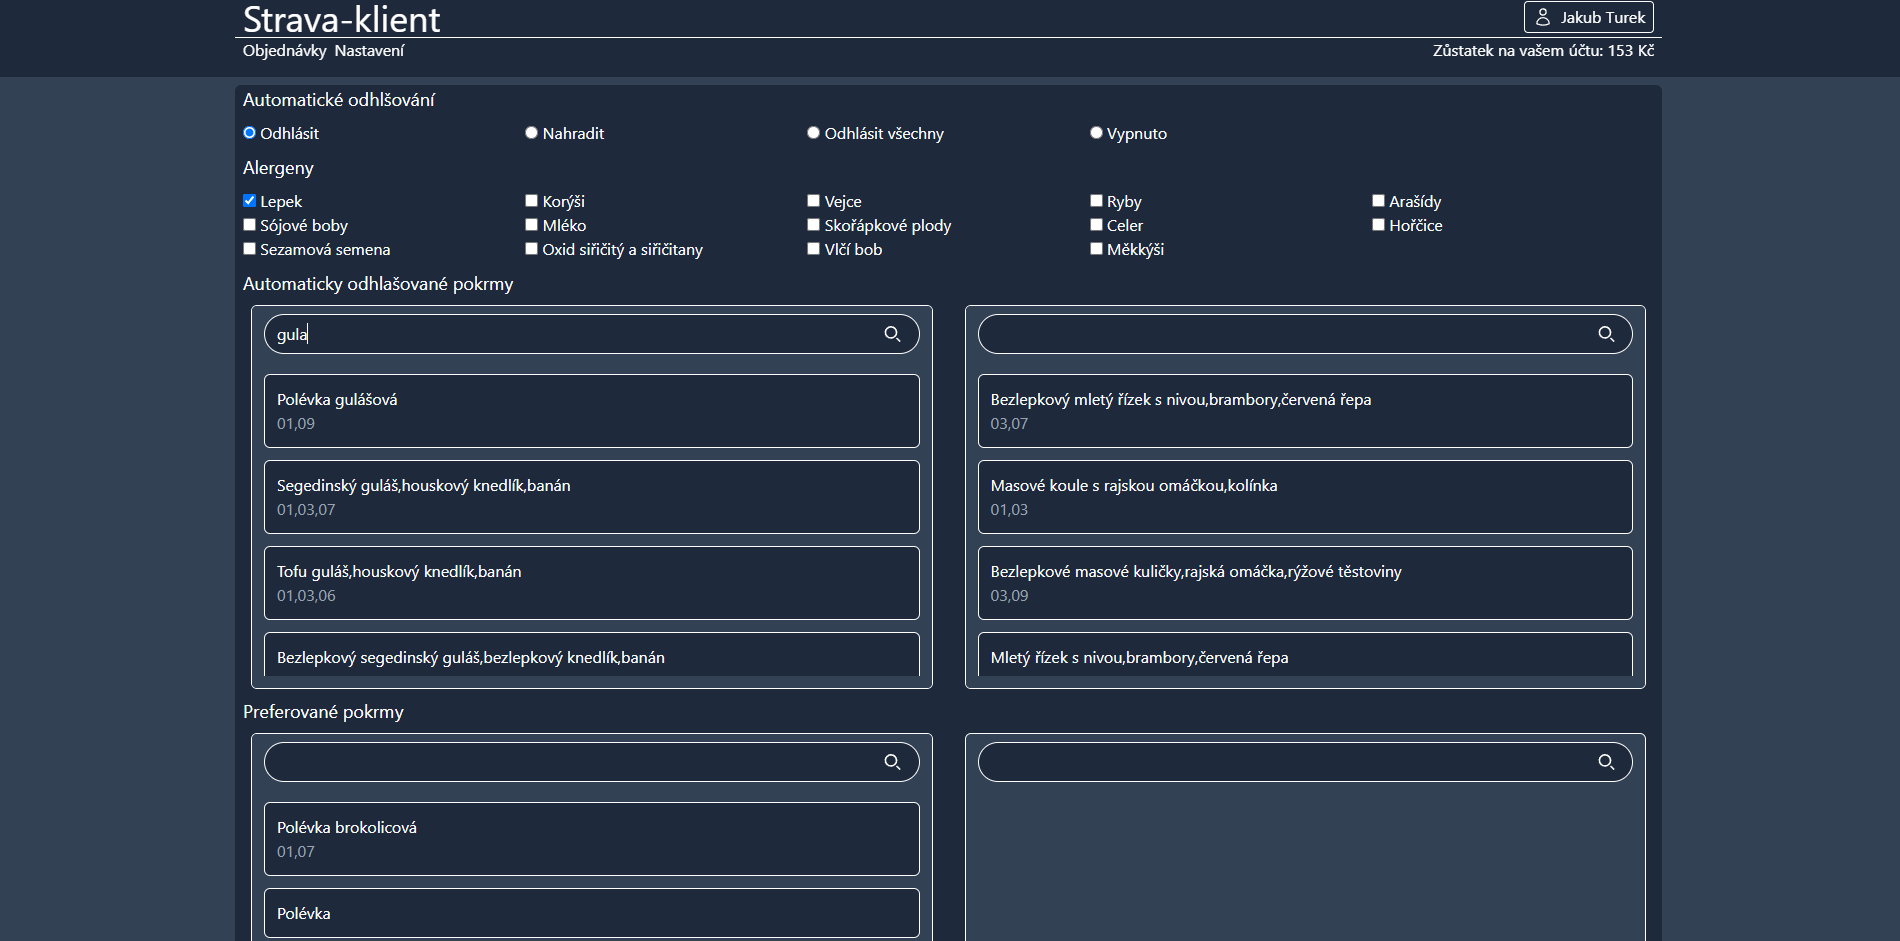
\includegraphics[scale=0.75, width=15cm]{pictures/settings.png}\par
\caption{Stránka nastavení s použitým vyhledáváním}
\end{listing}

Projekt zároveň využívá výhod SvelteKit frameworku jako jsou komponenty, které umožňuji snadné generovaní obsahu obsahující opakující se šablonu, jako je například právě jídelníček. Nebo reaktivní proměnné, které zajistí automatické znovu vykreslení na nich závislého obsahu\cite{reactive}, či story\cite{store}, které zase umožňuji zachovat reaktivitu společně se zachováním stavu při přechodu mezi jednotlivými stránkami\cite{store-sync}.

\newpage

\section{Klíčové problémy a jejich řešení}
Následující kapitola nastiňuje hlavní problémy řešené vrámci projektu a stručně popisuje princip jejich řešení

\subsection{Získávání dat z originální aplikace}
Jak již bylo zmíněno v úvodu, projekt dle původního zadání počítal se získávání dat z originální aplikace pomocí web scraperu. V té době aplikace ještě fungovala na principu rendrováni na straně serveru a bylo proto snadné, vzít výsledný html dokument a pomocí CSS selektorů získat potřebná data ze statické šablony. V průběhu vývoje tohoto projektu však aplikace přešla na renderování na straně klienta, což udělalo samotné získávání dat méně efektivní, jelikož bylo třeba potřebné elementy nejprve vykreslit. Z tohoto důvodu byla přidána ještě druhá metoda získávání dat a to prostřednictvím api oficiální aplikace, kdy jsou jednoduše vytvářeny požadavky na api a výsledný JSON je převeden do objektové reprezentace užívané v rámci celého projektu. Následující text tak popisuje základy fungování obou zmíněných metod.

\subsubsection{Web scraper}
Původně zamýšlená metoda získávání dat spoléhala na získávání dat přímo z výsledného html dokumentu pomocí CSS selektorů\cite{selector}, pomocí kterých byly lokalizovány elementy obsahující potřebná data ve statické šabloně použivatelné originální aplikací.

Jak již bylo zmíněno tato metoda však musela být v průběhu vývoje změněna, jelikož došlo k přechodu originální aplikace na vykreslování na straně klienta. Tato upravená verze tak nejprve opět lokalizuje podle selektorů potřebné elementy, s tím rozdílem, že je následně nejprve vykreslí a až poté dochází k získání dat z výsledného elementu stejným způsobem\cite{scraping}, jako tomu bylo u původní verze. Pro vykreslování jednotlivých elementů je využíván webový prohlížeč Firefox v headless verzi, ke kterému je prostřednictvím Marionette driveru\cite{marionette} připojen Geckodriver\cite{gecko}, jehož prostřednictvím je prohlížeč ovládán pomocí knihovny Fantoccini\cite{fantoccini}.

\subsubsection{Api}
Druhá z metod získávání dat je z oficiálního api. Tato metoda byla přidána v reakci na nutnost začít vykreslovat jednotlivé elementy pro extrakci dat, což přineslo snížení efektivity získávání dat po straně výkonu. Z tohoto důvodu bylo rozšířeno využívání oficiálního api, které bylo do této doby využíváno pouze pro měnění stavu oficiální aplikace (správa objednávek a podobně), také o možnost získávat jeho prostřednictvím potřebná data. 

Možnost nastavení aliasů v knihovně Serde\cite{alias} využívané pro serializaci dat v rámci projektu zároveň dělá převedení dat získaných ve formátu JSON z api do objektové reprezentace užívané napříč celým projektem a je tak možné dle potřeby přepínat mezi metodami získávání dat úpravou konfiguračního souboru \textit{config.toml}. Ve výchozím nastavení je preferováno využití api vzhledem k jeho vyšší efektivitě.

\subsection{Komunikační vrstvy}
Dálším z klíčových problémů bylo najít způsob, jak využít stejnou frontendovou aplikaci jak jako frontend pro webovou verzi projektu, tak pro uživatelské rozhraní desktopové aplikace bez nutnosti větších modifikací samotné aplikace pro tato použití.

Asi nejjednodušší řešením tohoto problému bylo využít možnosti frameworku SvelteKit před vykreslit statické části aplikace během jejího sestavování a následně je na straně klienta dynamicky doplňovat o dynamický obsah. Toto nastavení projektu pro využití společně s Tauri doporučuje i oficiální dokumentace. Tak nastavený projekt je zároveň možné využít i pro běžné nasazení v prostředí webu.

Pro použití aplikace v daném prostředí pak tedy stačí změnit skripty zajištující do vykreslení dynamického obsahu. To je zajištěno pomocí dvou TypeScriptových modulů \textit{TauriComunicationLayer} a \textit{WebComunicationLayer}, které exportují stejnou sadu funkcí obsluhující údálosti jako přihlášení, či načtení jídelníčku a pro úpravu aplikace pro dané prostředí tak stačí použít import těchto funkcí z příslušného modulu.

Co se týče fungování samotných modulů, webový modul využívá standartní JavaScript fetch api pro vytváření požadavků na backend webové aplikace. V případě modulu pro Tauri framework je použito Tauri invoke api, které vytváří požadavky lokálně obslouženy desktopovou aplikací\cite{invoke}. Následující ukázka kód znázorňuje vyvolání požadavku pro přhlášení pomocí Tauri invoke api.

\begin{listing}[!ht]
\begin{minted}{js}
const login = async (username: string, value: string, cantine: number) 
: Promise<Result<User,string>> =>{
    let res = await invoke('login', {
        username: username,
        password: value,
        cantine: cantine,
    })
    .then(
       (response) => {
           return {_t:'success', data: response as User} 
           as Success<User>;
       }
    ).catch(
        (error) => {
             return error as Failure<string>;
        }
        
    );
    return res; 
    
}
\end{minted}
\caption{Příklad vyvolání události z frontendu s použitím Tauri invoke api}
\end{listing}

\subsection{Historie jídelen}
Pro usnadnění vytváření seznamů preferovaných a zakázaných jídel vytváří aplikace historii jídelen, kdy periodicky prochází jídelničky jednotlivých jídelen a na jejich základě vytváří historii pro všechny jídelny v systému. Přesný způsob ukládaní této historie do databáze bude popsán v následující kapitole, nyní nicméně přejděme k fungování samotného získávaní dat pro vytváření historie.

Pro získávání dat se používá crawler script, který periodicky prochází jídelníčky jednotlivých jídelen, které jsou dostupné v oficiální aplikaci i bez nutnosti autentizace. Script je spouštěn na backendu webové aplikace s intervalem jednoho dne, k čemuž je využíváno specializované knihovny pro běhové prostředí Tokio inspirované démonem Cron\cite{cron}. Skript tak následně nejprve získá seznam všech jídelen v systému a poté iteračně stahuje jídelníček pro každou z jídelen, k získávaní dat se používá stejné metody, jako při získávání jídelníčku uživatele s pomocí api, a získaná data předá klientu databáze, který zajistí aktualizaci historie uložené pro danou jídelnu, zde je pro vetší efektivitu opět využíváno agregačních funkcí databáze pro práci s množinami.
\subsection{Ukládání dat a struktura databáze}
Následující kapitola stručně nastiňuje rozsah dat ukládaných aplikací a způsob jejich reprezentace v databázi. Z hlediska logického uspořádání by se data ukládaná aplikací dala rozdělit do dvou vetších celku data týkající se uživatelů a data o jídelnách v sytému. 

Začněme tedy od dat ukládaných aplikací týkajících se samotných uživatele. V tomto ohledu se oprojekt snaží minimalizovat množství ukládaných dat a ukládá proto pouze identifikátor uživatele, což je textový řetězec skládající se z uživatelského jména a jídelny u níž má uživatel účet, a nastaveni automatické správy objednávek, MongoDB umožňuje ukládat pole a objekty jako jednotlivé záznamy, pro přehlednost jsou v diagramu uložené objekty nahrazeny one-to-one vztahem a pole jiných než primitivních typu, jako v případě alergenů, one-to-many vztahy. Co se struktury samotného nastavení týče skládá se celkem ze dvou seznamů, které obsahují identifikátory odkazující na objekty jednotlivých jídel, samotná jídla jsou reprezentována názvem a seznamem alergenů, a představují oblíbená a zakázaná jídla uživatele. Dalším seznamem je seznam textových řetězců, představující zakázané alergeny. Posledním atributem je strategie, což je textový řetězec modifikující chování automatického klientu.

Pro jednotlivé jídelny je ukládán jejich identifikátor v systému Stravy.cz, který slouží primárně pro vnitřní komunikaci,jejich název, který je zobrazován uživatelům a také jejich historie. Historie je opět reprezentována seznamem odkazů na  objekty jednotlivých jídel. 

\begin{listing}[!ht]
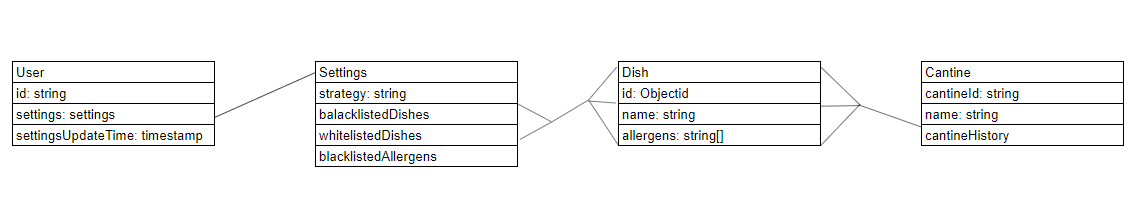
\includegraphics[scale=0.75, width=15cm]{pictures/schema.png}\par
\caption{Diagram znázorňující schéma databáze}
\end{listing}

\subsection{Automatický klient}
Jednou z klíčových funkcí aplikace je automatická správa objednávek, ta je implementována z pomocí automatického klienta. Celý automatický klient je postaven na základě běžného klienta používaného pro obsluhu událostí vyvolaných uživatelem, s tým rozdílem, že události jsou vyvolány na základě zpracování nastavení automatického klienta.

Jak již bylo řečeno klient v základu podporuje čtyři základní verze fungování. První z nich je vypnuto a asi není třeba vysvětlovat, že v tomto módu jednoduše nedochází ke spouštěni automatické správy objednávek. Výchozím režimem je režim odhlásit, kdy zkrátka dojde k odhlášení všech objednávek obsahující zakázané alergeny, či se nacházející na seznamu neoblíbených jídel. Vzhledem k nutnosti během procesu vyhodnocování předvoleb automatické správy je nutné pracovat i s aktuálními daty jídelníčku uživatele, které nejsou uloženy v databázi není možné využít výhod jejích agregačních funkcí a je proto využíváno množinových operací v rámci jazyka Rust. V tomto případě nejdříve dojde ke kontrole, zda seznam neoblíbených jídel neobsahuje aktuálně přihlášené jídlo, a v případě, že tomu tak není, dojde ještě ke kontrole, zda je průnik množiny zakázaných alergenů a alergenů v daném jídle prázdná množina. Pokud jeden z těchto testů skončí negativně, je objednávka zrušena a případně je stejná kontrola provedena pro další den.

Další z režimů je odhlásit a nahradit, v tomto režimu probíhá vyhodnocování podobně, jako v předchozím režimu stým rozdílem, že nejprve dojde ke kontrole, zda není průnik oblíbených jídel a denní nabídky prázdná množina, v případě, že denní nabídka obsahuje alespoň jeden preferovaný pokrm je jím nahrazena stávající objednávka, pokud také sama není na seznamu oblíbených jídel. Dále už vyhodnocení probíhá stejným způsobem jako v předchozím případě. V případě, že však dojde ke zrušení objednávky, je jsou pomocí rozdílu množin nalezena jídla, která jsou v denní nabídce a nejsou na seznamu zakázaných jídel, dojde ke kontrole alergenu, a pokud existuje alespoň jedno vyhovující jídlo v denní nabídce je jím aktuální objednávka nahrazena.

Posledním z režimů je režim odhlas všechny, který jednoduše zruší všechny zadané objednávky.

Vzhledem k tomu, že pro provádění akcí jménem uživatele je nutná autentizace, dochází ke spouštění automatického klienta v případě webové aplikace pouze v případě, že se uživatel k aplikaci přihlásí. Jí zadané údaje jsou následně použity k ověření identity a během načítání dat webu je na pozadí spuštěn automatický klient. V případě desktopové aplikace dochází k uložení údajů uživatele do systémového keychainu odkud jsou později vyzvednuty při startu systému a spuštění skriptu automatické správy objednávek.
\newpage
\section{Instalace}
Následující kapitola popisuje postup pro nasazení webové aplikace a instalace její desktopové verze.

Díky použití Dockeru a reverzní proxy Traefik je nasazení webové aplikace velice jednoduché stačí pouze nainstalovat Docker ve verzi podporující Docker Compose (některé distribuce ho nepodporují v základní verzi a je třeba ho doinstalovat) a provést minimální konfiguraci v souboru \textit{docker-compose.yaml}. Hodnoty potřebné nakonfigurovat a jejich význam znázorňuje následující tabulka.
\begin{listing}[!ht]
\begin{tabular}{ |p{5.7cm}|p{1.9cm}|p{6cm}| }
\hline
\multicolumn{3}{|c|}{Konfigurovatelné parametry webové aplikace} \\
\hline
Název& typ& popis\\
\hline
traefik.http.routers.*.rule=Host& label& adresa s platným DNS záznamem typu A s IP adresou hostitelského zařízení \\
\hline
traefik.http.services.*-https.loadbalancer.server.port& label& port docker kontejneru na, který jsou přesměrovávány požadavky - netřeba měnit pokud se port shoduje s portem definovaným v \textit{Dockerfile} kontejneru \\
\hline
certificatesresolvers.myresolver. acme.email& command& email používaqný pro zíkání SSL certifikátu od Let's Encrypt \\
\hline
/usr/api/certs/cert.pem& volume& cesta k autentifikačnímu certifikátu MongoDB \\
\hline
CONNECTION\_STRING& enviroment& connection string pro připojení k existujícímu MongoDB clusteru \\
\hline
PORT& enviroment& port, na kterém poslouchá backend webové aplikace \\
\hline
\end{tabular}
\caption{Seznam konfigurovatelných parametrů webové aplikace s jejiích popisem}
\end{listing}
Jak je již zřejmé z informací ve výchozí tabulce, projekt v současné konfiguraci počítá s připojením k databázi v již existujícím MongoDB Atlas clusteru, který lze snadno bezplatně vytvořit s pomocí oficiálního návodu\cite{atlas} a poté pouze zvolit možnost připojení pomocí certifikátu X.509, uložit vygenerovaný certifikát a cestu k němu společně s connection stringem uložit do konfiguračního souboru.

Ve výchozí formátu je konfigurační soubor \textit{docker-compose.yaml} nastaven pro vytvoření kontejnerů z kódu obsaženého v tomto repozitáři, v případě, že preferujete využití oficiálních již vytvořených imagů nahraných na Docker Hubu, je třeba \\\newline nahradit příslušné řádky v sekcích \textit{image} a \textit{build} dle komentářů v konfiguračním soubor.

Po dokončení konfigurace s pomocí výše zmíněných informací a instrukcích v komentářích konfiguračního souboru již stačí jen spustit všechny kontejnery pomocí následujícího příkazu.

\begin{listing}[!ht]
\begin{minted}{shell}
docker compose up -b
\end{minted}
\caption{Příkaz pro spuštění kontaineru webové aplikace}
\end{listing}

Pro instalaci desktopové aplikace stačí stáhnout, buďto installer pro operační systém Windows, který stačí po stažení pouze spustit a projít procesem instalace, nebo balíček \textit{.deb} umožnující spuštění na distribucích Linuxu založených na distribuci Debian, či spustitelný Appimage pro ostatní distribuce Linuxu, v sekci Releases v tomto GitHub repozitáři.
\newpage
\section{Závěr}
Závěrem přejděme k celkovému zhodnocení výsledného projektu a možnostem jeho dalšího směřování a případným budoucím vylepšením.

Celkově by se projekt dal považovat za úspěšný, jelikož splňuje všechny cíle stanovené v zadání a jeho finální verze obsahuje nad rámec zadání i možnost získávat data z oficiální aplikace přímo prostřednictvím oficiálního api, jejíž přidání bylo spíše kompromisem mezi dodržením podoby aplikace stanovené v zadáním a dosažením lepších výsledků po stránce výkonu, po přechodu oficiální aplikace na vykreslování na straně klienta a uživatel se tak může rozhodnout, zda chce používat původní způsob získávaní dat využívající web scraperu, či novou verzi s lepšími výsledky po stránce výkonu.

Z hlediska možných vylepšení se nabízí další vylepšení a zpřehlednění uživatelského rozhraní aplikace a případné předělání webové aplikace do podoby, kdy bude plně využívat pouze vykreslování na straně serveru, což by uživatelům přineslo o něco plynulejší a pohodlnější uživatelský zážitek, ale zároveň zkomplikovalo integraci s desktopovou verzí aplikace.

Dále se nabízí možnost vytvoření systému notifikací, které by uživateli umožnili, dostávat ve stanoveném intervalu, například jednoho týdne, informace o fungování automatické správy objednávek a poskytli mu lepší přehled o jeho fungování.
\newpage
\printbibliography[heading=bibintoc,title={Reference}]
\newpage
\addcontentsline{toc}{section}{Seznam příloh}
\listoflistings


\end{document}
